\subsection{Changing $\alpha_k$}\label{subsec:changing-alpha-k}
In this section we will discuss the results from the experiments made with the methods that where described in \autoref{sec:method:alpha-k-effect}.
\begin{itemize}
    \item \textbf{RQ1}: How does changing $\alpha_k$ affect the performance in LightGCN?
\end{itemize}

\subsubsection{Removing $\alpha_k$}\label{subsubsec:remove-alpha-k}
The results from running the experiment on the yelp2020 dataset can be seen on \autoref{fig:ndcg-yelp2020-alpha-k}.
It shows that removing $\alpha_k$ was detrimental for the performance.
In the initial epochs, LightGCN $\alpha_k = 1$ (LightGCN-Ak1) performs better, but it quickly starts to decline in performance.
The results from amazon-book are similar and can be seen in \autoref{app:removing-alpha-k}
These results indicates that $\alpha_k$ is an important part of the layer combination for weighted summation, and that summation is not beneficial for LightGCN.
\begin{figure}
    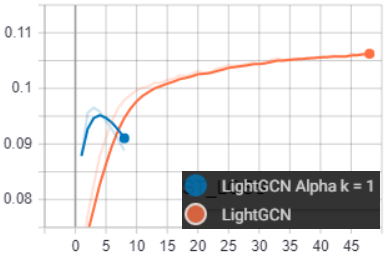
\includegraphics[width=\linewidth]{figures/alpha-k-results/yelp2020-ndcg.png}
    \caption{NDCG@50 of LightGCN and LightGCN-Ak1 on yelp2020}
    \label{fig:ndcg-yelp2020-alpha-k}
\end{figure}

\subsubsection{Utilizing only one layer}
In this section we experiment with removing the layer combination, and only utilizing the embedding from a specific convolution layer.
This method is described in \autoref{subsubsec:only-1-layer}.
$\mathbf{e}^{(0)}$, $\mathbf{e}^{(1)}$, $\mathbf{e}^{(2)}$, $\mathbf{e}^{(3)}$, $\mathbf{e}^{(4)}$ and $\mathbf{e}^{(5)}$ are used as the final embeddings in each experiment.
These are compared to LightGCN where weighted sum is utilized with a different number of layers.
\begin{table*}[]
    \centering
    \begin{tabular}{|l|l|l|l|l|l|l|}
        \hline
                             & \multicolumn{2}{l|}{Amazon-Cell-Sport} & \multicolumn{2}{l|}{Yelp2020} & \multicolumn{2}{l|}{Amazon-Book}                                                                 \\ \hline
                             & NDCG@50                                & Recall@50                     & NDCG@50                          & Recall@50         & NDCG@50             & Recall@50           \\ \hline
        Weighted sum (1 con) & 0.02804                                & 0.05503                       & 0.0969                           & 0.1955            & 0.0427              & 0.07408             \\ \hline
        Weighted sum (2 con) & 0.03132                                & 0.06133                       & 0.1008                           & 0.2015            & 0.0463              & 0.08055             \\ \hline
        Weighted sum (3 con) & 0.03237                                & 0.06447                       & 0.1064                           & 0.2106            & \textbf{0.04668}    & \textbf{0.08129}    \\ \hline
        Weighted sum (4 con) & 0.03253                                & 0.06394                       & 0.1084                           & 0.2157            & \underline{0.04617} & \underline{0.08033} \\ \hline
        Weighted sum (5 con) & 0.03285                                & 0.06451                       & \textbf{0.1089}                  & \textbf{0.2177}   & 0.04515             & 0.07861             \\ \hline
        $\mathbf{e}^{(0)}$   & 0.02169                                & 0.04447                       & 0.08177                          & 0.1674            & 0.03669             & 0.06373             \\ \hline
        $\mathbf{e}^{(1)}$   & 0.02523                                & 0.04859                       & 0.1019                           & 0.2039            & 0.0458              & 0.079               \\ \hline
        $\mathbf{e}^{(2)}$   & 0.03419                                & 0.06809                       & \underline{0.1086}               & \underline{0.217} & 0.04487             & 0.07755             \\ \hline
        $\mathbf{e}^{(3)}$   & 0.03483                                & 0.06972                       & 0.09956                          & 0.2001            & 0.0372              & 0.06412             \\ \hline
        $\mathbf{e}^{(4)}$   & \underline{0.0366}                     & \textbf{0.07377}              & 0.08863                          & 0.1788            & 0.03247             & 0.05607             \\ \hline
        $\mathbf{e}^{(5)}$   & \textbf{0.03733}                       & \underline{0.07318}           & 0.0819                           & 0.1643            & 0.02923             & 0.05022             \\ \hline
    \end{tabular}
    \centering
    \caption{Experiment on LightGCN where different layers are used as the final embedding compared with weighted sum.}
    \label{tab:only-use-one-layer-experiment}
\end{table*}
As can be seen on \autoref{tab:only-use-one-layer-experiment} the results vary a lot depending on the dataset.
For Amazon-Cell-Sport only considering $e^{(4)}$ and $e^{(5)}$ gives the best results which perform around 13 \% better than weighted sum with 5 convolutions.
This could be because Amazon-Cell-Sport consists primarily of nodes with few interactions, and therefore the later convolutions have the largest impact. 
90 \% of all items within this dataset have 5 interactions, which is one of the reasons that the later convolutions perform so well.
For Yelp2020 the best results were weighted sum with 5 convolutions closely followed by $e^{(2)}$.
This dataset varies more in terms of the number of interactions that the users have.
For Amazon-Book weighted sum with 3 convolutions performs best and this could be because there is a large variation of how many interactions the users have.
One of the advantages of weighted sum is that it stabilizes the results.
This might have a positive effect in some cases compared to our method where we only use the embedding from one of the layers.
From this we can conclude that for datasets, where items or users generally have few connections it is worth considering only using $e^{(4)}$ or $e^{(5)}$ instead of using weighted sum.

\subsubsection{Removing 0th layer}
The final method that we described in \autoref{sec:method:alpha-k-effect} was removing the 0th layer embedding before combining the embeddings from the different layers.
In this subsection we show results from the experiments done with this method.
\begin{table*}[h!]
    \centering
    \begin{tabular}{|l|l|l||l|l||l|l|}
        \hline
                            & \multicolumn{2}{c||}{Recall@50}           & \multicolumn{2}{c||}{NDCG@50}             \\ \hline
        Method              & 5 con average     & $E^{(0)}$ removed     & 5 con average       & $E^{(0)}$ removed   \\ \hline
        Amazon-Cell-Sport   & 0.06451           & \textbf{0.06726}      & 0.03285             & \textbf{0.03460}             \\ \hline
        Yelp2020            & \textbf{0.2177}   & 0.21289               & \textbf{0.1089}     & 0.10641            \\ \hline
        Amazon-Book         & \textbf{0.08129}  & 0.07715               & \textbf{0.04668}    & 0.04470            \\ \hline
    \end{tabular}
    \label{tab:removing-0th-layer-embedding-experiment}
    \caption{Results from experiment where we remove 0th layer embedding}
\end{table*}
While Amazon-Cell-Sport has an improved performance when the 0th embedding is removed, the other datasets see a decrease in performance.
